%%
%  ******************************************************************************
%  * #file    Szablon_raportu_EN_Latex.tex
%  * #author  Adrian Wójcik   adrian.wojcik(at)put.poznan.pl
%  *          
%  * #commit  Patryk Kościk   koscikpatryk(at)gmail.com
%  *          Modified the template for Projekt przejsciowy purposes          
%  *          
%  *
%  * #commit  Patryk Kościk   koscikpatryk(at)gmail.com
%  *          Zupełnie przewrócono na łeb formatke po taktycznym wyjasnieniu          
%  *          
%  * #version 1.1
%  * #date    09-Mar-2022
%  * #brief   PROJPRZEJ
%  *
%  ******************************************************************************
%%  
\documentclass[11pt, a4paper]{article}

\usepackage{SM_template}

% Wypełnijcie te dyrektywy zgodnie z waszym tematem
%
% \lab      -> NAZWA CZUJNIKA,          np.: 'DHT22'
% \comment  -> Króciutki opis co to,    np.: 'Cyfrowy czujnik temperatury'
% \author   -> Autor dokumentu          np.: Patryk Kościk
%
% Pamiętajcie o zmianie ścieżki w \addbibresourcue (!)

\lab{Moduł MAX30100}
\comment{Czujnik tętna i natężenia tlenu we krwi}
\author{Anna Nasierowska}
\addbibresource{bib/MAX30100.bib}

%
% Początek dokumentu
%
\begin{document}

%
% Strona tytułowa
%
\mainpage{fig/MAX30100/tytul.png}
\newpage

\section*{Opis elementu}
Cały moduł opiera się sensorze optycznym, który odbiera światło czerwone i podczerwone, wydostające się z umieszczonych obok czujnika diod o wysokim natężeniu światła. Sensor odbiera fale o długości 660nm dla światła czerwonego oraz 880nm dla światła podczerwonego. Razem z diodami znajduje się on w 14 pinowym układzie scalonym, umożliwiającym komunikację z mikrokontrolerem przez magistralę $I^2C$ oraz samodzielne sterowanie diodami(opcjonalne). 

%%%%%%%%%%%%%%%%%%%%%%%%%  TWO IMAGES SIDE BY SIDE  %%%%%%%%%%%%%%%%%%%%%%%%%%%%%
\vspace{0.25cm}
\begin{figure}[h]
\centering
%%%%%%%%%%%%%%%%%%%%%%%%%%%%%%%%%%%%%%%%%%%%%%%%%%%%%%%%%%%%%%%%%%%%%%%%%%%%%%%%%
\begin{subfigure}{.5\textwidth}
\centering
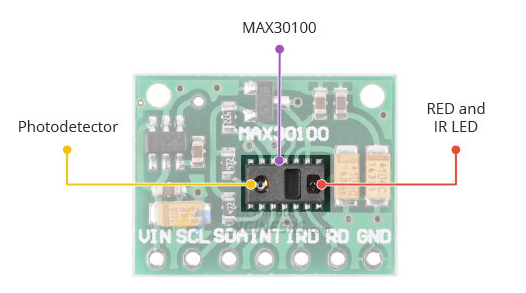
\includegraphics[width=\linewidth]{fig/MAX30100/zdj_modułu/czujnik.png}
\caption{Zdjęcie modułu z zaznaczonym czujnikiem}
\label{fig:_zdjecie_elementu}
\end{subfigure}%
%%%%%%%%%%%%%%%%%%%%%%%%%%%%%%%%%%%%%%%%%%%%%%%%%%%%%%%%%%%%%%%%%%%%%%%%%%%%%%%%%
\begin{subfigure}{.5\textwidth}
\centering
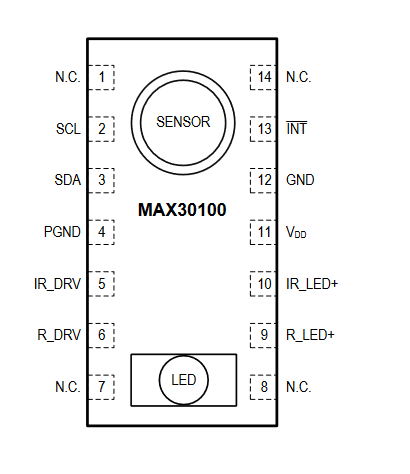
\includegraphics[width=.5\linewidth]{fig/MAX30100/zdj_modułu/czujnik_rys.png}
\caption{Schemat obudowy czujnika MAX30100 z pinoutem.}
\label{fig:_zasada_dzialania_elementu}
\end{subfigure}
%%%%%%%%%%%%%%%%%%%%%%%%%%%%%%%%%%%%%%%%%%%%%%%%%%%%%%%%%%%%%%%%%%%%%%%%%%%%%%%%%
% \caption{PODPIS}
\label{fig:element}
\end{figure}
\vspace{0.25cm}
%%%%%%%%%%%%%%%%%%%%%%%%%  TWO IMAGES SIDE BY SIDE  %%%%%%%%%%%%%%%%%%%%%%%%%%%%%



% \subsection{Opis modułu} REPLACE SUBSECTION WITH 1CM VSPACE
\vspace{0.75cm}

Moduł omawiany w tym dokumencie, to nieco bardziej skomplikowany układ, składający się z 7 kondensatorów, 3 rezystorów, regulatorów napięcia zasilania (U1 - 6pinowy układ scalony oraz U2 - 3 pinowy układ scalony) oraz układu scalonego z czujnikiem i LED'ami. Ma on 7 wyprowadzeń: 
\begin{itemize}
    \item VIN oraz GND - służą do zasilania modułu w zakresie 3.3-5V. 
    \item SCL oraz SDA - służą do komunikacji z mikrokontrolerem za pomocą interfejsu $I^2C$
    \item IRD oraz RD  - do sterowania diodami, kolejno podczerwoną i czerwoną
    \item INT - do obsługi przerwań 
\end{itemize}

%%%%%%%%%%%%%%%%%%%%%%%%%  TWO IMAGES SIDE BY SIDE  %%%%%%%%%%%%%%%%%%%%%%%%%%%%%
\begin{figure}[h]
\centering
%%%%%%%%%%%%%%%%%%%%%%%%%%%%%%%%%%%%%%%%%%%%%%%%%%%%%%%%%%%%%%%%%%%%%%%%%%%%%%%%%
\begin{subfigure}{.5\textwidth}
\centering
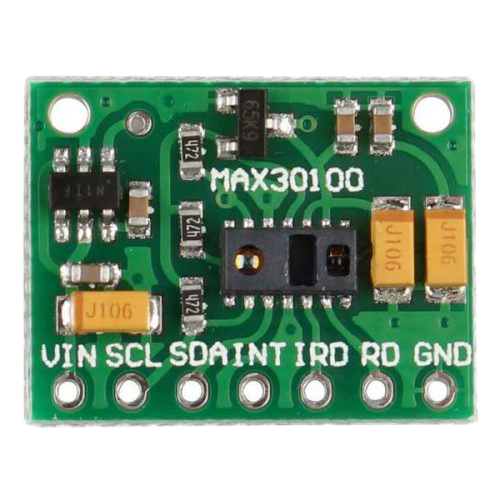
\includegraphics[width=.5\linewidth]{fig/MAX30100/zdj_modułu/zdj.png}
\caption{Zdjęcie modułu}
\label{fig:_zdjecie_modulu}
\end{subfigure}%
%%%%%%%%%%%%%%%%%%%%%%%%%%%%%%%%%%%%%%%%%%%%%%%%%%%%%%%%%%%%%%%%%%%%%%%%%%%%%%%%%
\begin{subfigure}{.5\textwidth}
\centering
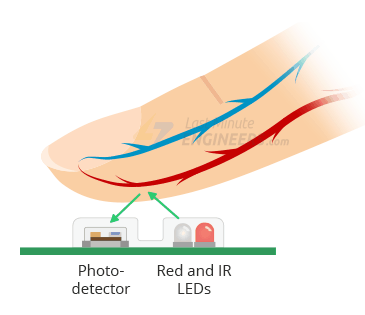
\includegraphics[width=.6\linewidth]{fig/MAX30100/zasada_dzialania/zasada_dzial.png}
\caption{Sposób użycia modułu}
\label{fig:_schemat_modulu}
\end{subfigure}
%%%%%%%%%%%%%%%%%%%%%%%%%%%%%%%%%%%%%%%%%%%%%%%%%%%%%%%%%%%%%%%%%%%%%%%%%%%%%%%%%
\label{fig:modul}
\end{figure}
\vspace{0.5cm}
%%%%%%%%%%%%%%%%%%%%%%%%%  TWO IMAGES SIDE BY SIDE  %%%%%%%%%%%%%%%%%%%%%%%%%%%%%

Pomiar tętna wykonywany przez czujnik opiera się na fakcie, że dotlenione hemoglobiny mają właściwości pochłaniające światło podczerwone. Kiedy naczynia krwionośne pompują krew, przesuwają dotlenione hemoglobiny powodując zmiany w ilości podczerwonego światła, które odbija się do sensora, tworząc w ten sposób graf przedstawiający tętno. \\
Dodatkowo nieutlenione hemoglobiny odbijają mniej światła podczerwonego, a za to więcej światła czerwonego. Zatem dzięki dołożeniu do czujnika tętna czerwonej diody możliwe jest oprócz tętna, zmierzenie światła odbijanego przez krwinki utlenione i nieutlenione z osobna. Mając takie informacje obliczana jest procentowa wartość tlenu we krwi. 
Czujnik o takim działaniu jest wykorzystywany w wielu nowoczesnych urządzeniach, takich jak pulsoksymetry do użytku domowego, szpitalnego czy np. w smartwatch'ach. 


\begin{figure}[h]
    \centering
    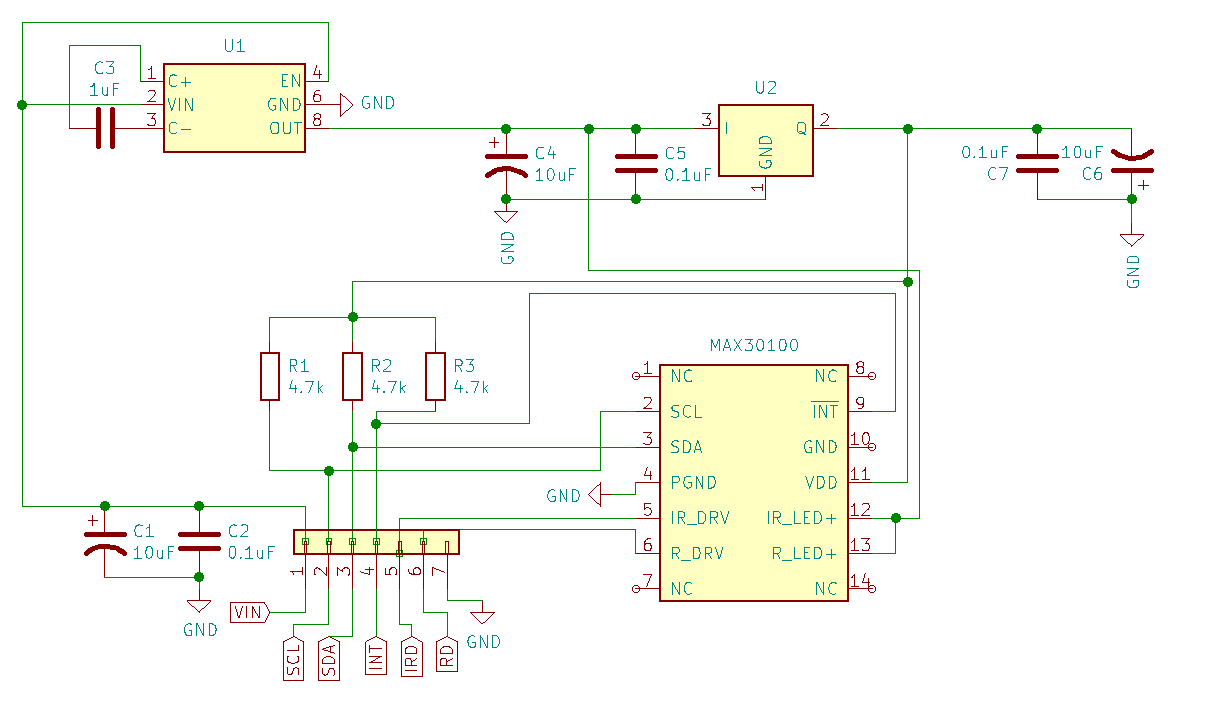
\includegraphics[width=0.8\textwidth]{fig/MAX30100/polaczenie_modulu/schemat.png}
    \caption{Połączenie układu}
    \label{fig:polaczenie_ukladu}
\end{figure}



\section{Użycie czujnika}

Moduł podłączono do płytki ARDUINO Uno za pomocą interfejsu $I^2C$ (piny A4 i A5) z rezystorami podciągającymi 10kOhm do napięcia 5V,  w sposób widoczny na zdjęciach:
\begin{figure}[h]
\begin{subfigure}{.5\textwidth}
\centering
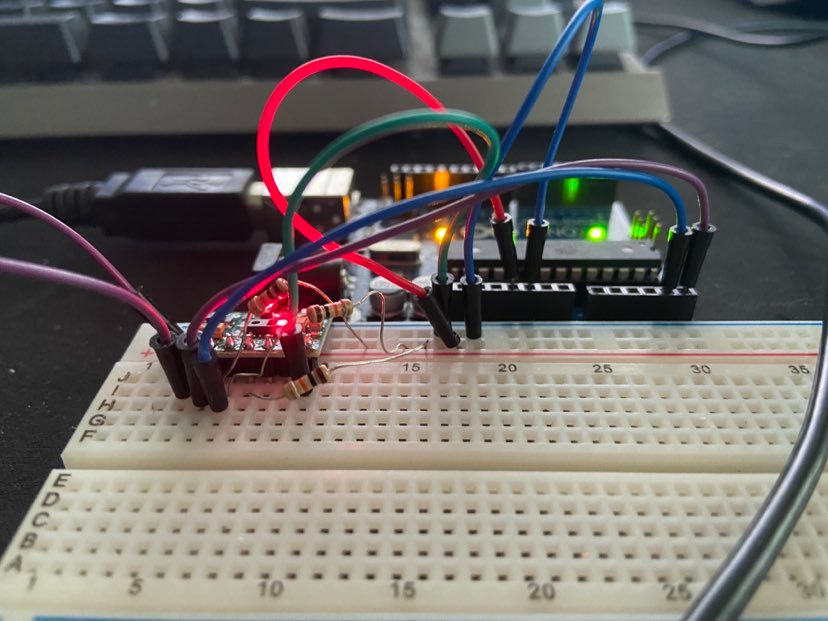
\includegraphics[width=\linewidth]{fig/MAX30100/działanie_ukladu/zdj1.jpg}
\label{fig:_zdjecie_elementu}
\end{subfigure}%
%%%%%%%%%%%%%%%%%%%%%%%%%%%%%%%%%%%%%%%%%%%%%%%%%%%%%%%%%%%%%%%%%%%%%%%%%%%%%%%%%
\begin{subfigure}{.5\textwidth}
\centering
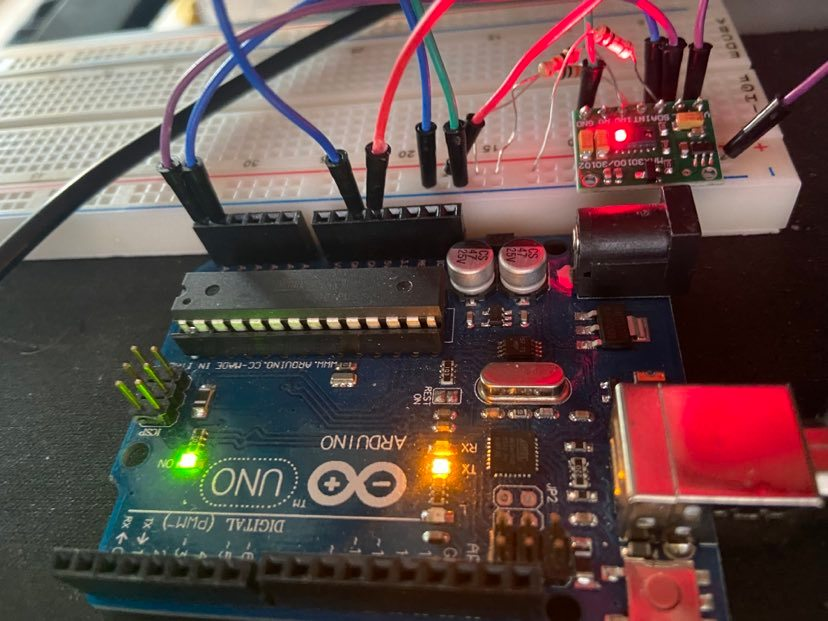
\includegraphics[width=\linewidth]{fig/MAX30100/działanie_ukladu/zdj2.jpg}
\label{fig:_zasada_dzialania_elementu}
\end{subfigure}
\end{figure}

Można zauważyć na zdjęciu mocno świecącą czerwoną diodę - to wspomniana wyżej dioda służąca do wykoniania pomiaru, która potwierdza również w sposób widoczny, że moduł jest podłączony prawidłowo i działa. Następnie w celu sprawdzenia działania czujnika wykonano pomiar tętna na palcu przedstawiony poniżej: 

\begin{figure}[h]
\centering
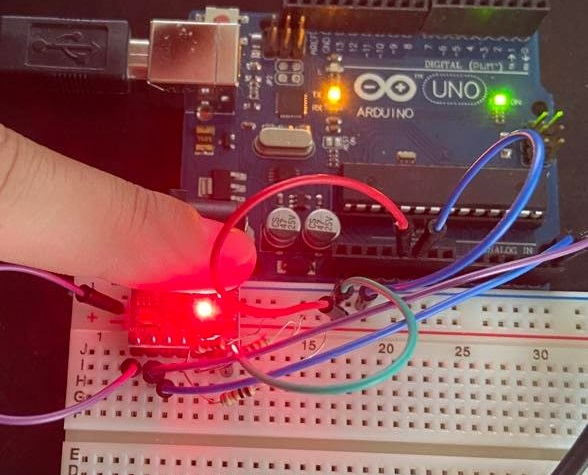
\includegraphics[width=0.5\linewidth]{fig/MAX30100/działanie_ukladu/zdj3.jpg}
\label{fig:_zasada_dzialania_elementu}
\end{figure}
%%%%%%%%%%%%%%%%%%%%%%%%%%%%%%%%%%%%%%%%%%%%%%%%%%%%%%%%%%%%%%%%%%%%%%%%%%%%%%%%%
\begin{figure}[h]
\centering
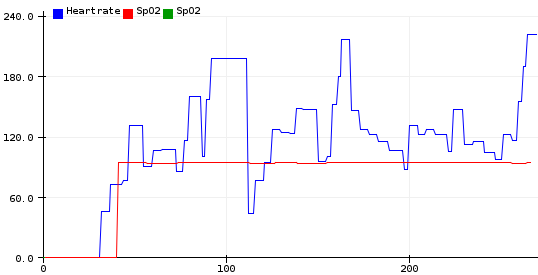
\includegraphics[width=\linewidth]{fig/MAX30100/działanie_ukladu/tętno_i_Spo.png}
\label{fig:_zdjecie_elementu}
\end{figure}




\newpage
\printbibliography[heading=bibintoc]

\end{document}